\section{Vorgaben}
\subsection{\eurobot}

\begin{frame}
	\setbeamercovered{transparent}
	\frametitle{\eurobot} % TODO besserer Titel: wie wärs mit Aufgaben?
	
	\begin{itemize}
		\item 1-2 Roboter pro Team
		\item Roboter bewegen sich autonom
		\item Behinderung und Beschädigung des Gegners ist nicht erlaubt
	\end{itemize}
	% Darum sind diverse Sensoren und die Gegnerekennung nötig
	
\end{frame}

\begin{frame}
	\frametitle{\eurobot}
	\framesubtitle{Spielfeld}
	
	\begin{figure}
	   	\centering
	   	\begin{tikzpicture}[scale=0.8, transform shape]
	   	\node[anchor=south west,inner sep=0] (image) at (0,0) {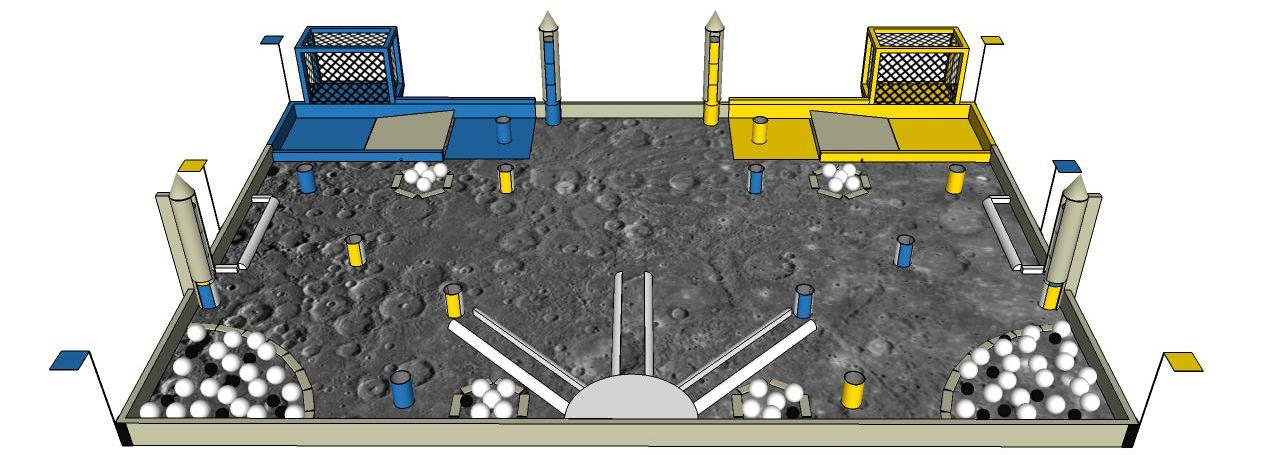
\includegraphics[width=\textwidth] {../images/spielfeldElemente.jpg}};
	   	\begin{scope}[x={(image.south east)},y={(image.north west)}]
	   	\draw [line width=0.4mm, ->, cGreen] (0.05,0.85) node[left, color=black]{\textit{cargo bay}} -- (0.235,0.85); 
	   	\draw [line width=0.4mm, ->, cGreen] (0.05,0.7) node[left, color=black]{Startfeld} -- (0.25,0.7); 
	   	\draw [line width=0.4mm, ->, cGreen] (0.05,0.55) node[left, color=black]{Rackete} -- (0.12,0.55); 
	   	\draw [line width=0.4mm, ->, cGreen] (0.05,0.4) node[left, color=black]{\textit{moon base}} -- (0.48,0.4); 
	   	\draw [line width=0.4mm, ->, cGreen] (0.05,0.25) node[left, color=black]{Krater} -- (0.14,0.25);
	   	
	   	\draw [line width=0.4mm, ->, cGreen] (0.95,0.9) node[right, color=black]{\textit{beacon}} -- (0.8, 0.9);
	   	\draw [line width=0.4mm, ->, cGreen] (0.95,0.7) node[right, color=black]{Wippe} -- (0.7, 0.7);
	   	\draw [line width=0.4mm, ->, cGreen] (0.95,0.52) node[right, color=black]{\textit{moon base}} -- (0.8, 0.52);
	   	\draw [line width=0.4mm, ->, cGreen] (0.95,0.13) node[right, color=black]{Krater} -- (0.62, 0.13);
	   	
	   	\end{scope}
	   	\end{tikzpicture}
	\end{figure}
\end{frame}

\begin{frame}
	\frametitle{\eurobot}
	\framesubtitle{\textit{Lunar Modules}}
	
	\begin{itemize}
		\item \textit{Lunar modules} seitwärts in die \textit{moon base} legen.
		\begin{itemize}
			\item mehrfarbige \textit{lunar modules} drehen, bis eigene Farbe oben ist
			% auch ins shuttle legen möglich
		\end{itemize}
	\end{itemize}

	\begin{figure}
		\begin{subfigure}{0.1\textwidth}
			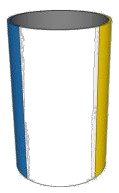
\includegraphics[width=\textwidth]{../images/lunarModuleMulticolor.jpg}
		\end{subfigure}
		\hspace{1em}
		\begin{subfigure}{0.1\textwidth}
			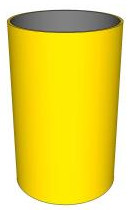
\includegraphics[width=\textwidth]{../images/lunarModule.jpg}
		\end{subfigure}
		\hspace{2em}
		\begin{subfigure}{0.5\textwidth}
			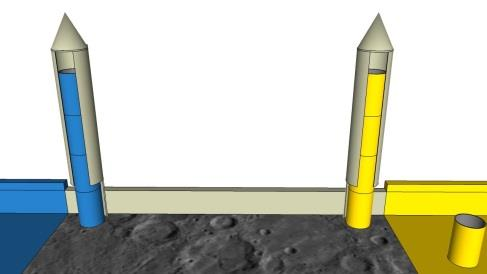
\includegraphics[width=\textwidth]{../images/rockets.jpg}
		\end{subfigure}
	\end{figure}

\end{frame}

\begin{frame}
	\frametitle{\eurobot}
	\framesubtitle{\textit{Titanium Ores}}
	
	\begin{itemize}
		\item \textit{Titanium ores} in \textit{cargo bay} befördern oder in den \textit{shuttle} legen
		% von Mondgestein trennen, da diese keine Punkte geben und im shuttle nur 10 Kugeln gezählt werden
	\end{itemize}
	
	\begin{figure}
		\begin{subfigure}{0.4\textwidth}
			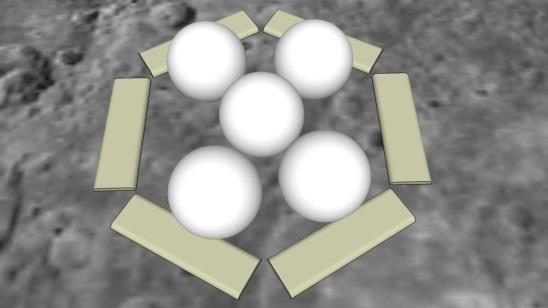
\includegraphics[height=2.5cm]{../images/craterSmall.jpg}
		\end{subfigure}
		\hspace{1em}
		\begin{subfigure}{0.4\textwidth}
			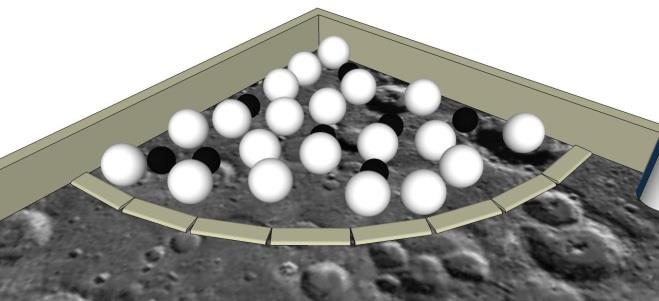
\includegraphics[height=2.5cm]{../images/craterBig.jpg}
		\end{subfigure}
	\end{figure}
	
\end{frame}


\subsection{SA-ES-350}
\begin{frame}
	\frametitle{Vorgaben SA-ES-350}
	
	\begin{itemize}
		\item Ausarbeitung der Konzepte der Roboter.
		\item Hauptkomponenten vom Vorjahr übernehmen und anpassen:
		\begin{itemize}
			\item Mainboard%: neue Hardware, Software vorbereiten
			\item Fahrcontroller%: Kurven fahren, einfachere Kalibrierung
			\item Gegnererkennung%: LED-Ring, Adapterboard, Software
		\end{itemize}
		
		\item Alle elektrischen Komponenten auswählen und bereitstellen.
	\end{itemize}

\end{frame}  
